\documentclass[12pt]{article}

\usepackage[a4paper,margin=1in]{geometry}
\usepackage{amsmath,amssymb}
\usepackage{newtxtext,newtxmath} % Times-style font
\usepackage{fancyhdr}
\usepackage{listings}
\usepackage{graphicx}
\usepackage{float}
\usepackage{algorithm}
\usepackage{algpseudocode}
\usepackage{booktabs}
\usepackage{xcolor}

\setlength{\textfloatsep}{10pt}
\setlength{\floatsep}{10pt}

\setlength{\parindent}{0pt}
\setlength{\parskip}{5pt}

% Keep entire document at 12 pt
\AtBeginDocument{
    \fontsize{12pt}{14pt}\selectfont
}

\lstdefinestyle{code}{
    language=Python,
    basicstyle=\ttfamily\fontsize{9.5pt}{11.5pt}\selectfont,
    breaklines=true,
    breakatwhitespace=false,
    frame=single,
    numbers=left,
    numberstyle=\tiny\color{gray},
    keywordstyle=\color{blue},
    commentstyle=\color{gray},
    stringstyle=\color{green!50!black},
    columns=fullflexible,
    keepspaces=true,
    showstringspaces=false
}

\lstdefinestyle{output}{
    basicstyle=\ttfamily\fontsize{9pt}{11pt}\selectfont,
    breaklines=true,
    breakatwhitespace=false,
    frame=single,
    numbers=none,
    backgroundcolor=\color{gray!6},
    columns=fullflexible,
    keepspaces=true,
    showstringspaces=false
}

% ------------------------------------------------
% Header
% ------------------------------------------------

\pagestyle{fancy}
\fancyhf{}

\fancyhead[L]{Name: Kishan Sahu{\hspace{4cm}}}
\fancyhead[R]{Enrollment No.: P26DS017{\hspace{3.5cm}}}

\renewcommand{\headrulewidth}{0.4pt}
\setlength{\headheight}{15pt}

% ------------------------------------------------
% Code formatting
% ------------------------------------------------

\lstset{
    basicstyle=\ttfamily\fontsize{9.5pt}{11.5pt}\selectfont,
    breaklines=true,
    frame=single,
    columns=fullflexible,
    keepspaces=true,
    showstringspaces=false
}

\begin{document}

% ------------------------------------------------
% TITLE
% ------------------------------------------------

\begin{center}
\textbf{Computer Science and Engineering Department, SVNIT, Surat}\\
\textbf{M.Tech. I -- Semester I}\\
\textbf{Machine Learning (CSDS105)}\\
\textbf{Lab Assignment 9: Logistic Regression for Text Classification and Multi-Algorithm Benchmarking}
\end{center}

\vspace{0.3cm}

\section{Introduction and Problem Formulation}

Text classification represents a critical capability across modern information systems, spanning automated spam detection, sentiment analysis, document routing, and content moderation. While deterministic linear hyperplanes (such as the Perceptron and Support Vector Machines explored in Labs 5 and 8) establish geometric separating surfaces, real-world decision pipelines frequently require calibrated posterior probabilities $P(Y = 1 \mid \mathbf{x})$ rather than binary step decisions.

\textbf{Logistic Regression} represents the foundational \textbf{discriminative probabilistic linear model} for binary classification. Grounded in maximum likelihood estimation and information theory, logistic regression models the posterior log-odds of a class as an affine combination of input features.

This laboratory assignment conducts a systematic empirical study using the Kaggle \textbf{SMS Spam Collection} corpus ($N = 5,572$ instances), executing three core investigations:
\begin{enumerate}
    \item \textbf{Implementation & Parameter Interpretability}: Fitting an $L_2$-regularized Logistic Regression model on sublinear TF-IDF features and analyzing the learned weight coefficients to identify the most predictive linguistic tokens.
    \item \textbf{Multi-Algorithm Benchmark}: Benchmarking Logistic Regression against three diverse classification paradigms:
    \begin{itemize}
        \item \textbf{Multinomial Naive Bayes (NB)}: A generative probabilistic model computing class-conditional joint likelihoods under word-independence assumptions.
        \item \textbf{Decision Tree Classifier}: A non-parametric eager recursive partitioner using information-theoretic splits.
        \item \textbf{K-Nearest Neighbors (KNN)}: An instance-based lazy learner using spatial Cosine distance metrics.
    \end{itemize}
    \item \textbf{Rigorous Quantitative Diagnostics}: Evaluating effectiveness across Accuracy, Precision, Recall, and the balanced F1-Score, supplemented by comparative bar charts and confusion matrix heatmaps.
\end{enumerate}

\subsection{Dataset Overview and Exploratory Inspection}
The corpus comprises $N = 5,572$ text messages categorized into legitimate communications (\texttt{ham}) and fraudulent promotions (\texttt{spam}). Table~\ref{tab:dataset_dist} summarizes the target distribution.

\begin{table}[H]
\centering
\caption{Target Class Distribution of the SMS Spam Dataset}
\label{tab:dataset_dist}
\vspace{0.2cm}
\begin{tabular}{lccc}
\toprule
\textbf{Class Label} & \textbf{Encoded Target} & \textbf{Instance Count} & \textbf{Percentage (\%)} \\
\midrule
Ham (Legitimate) & 0 & 4,825 & 86.59\% \\
Spam (Fraudulent) & 1 & 747 & 13.41\% \\
\midrule
\textbf{Total} & -- & \textbf{5,572} & \textbf{100.00\%} \\
\bottomrule
\end{tabular}
\end{table}

The severe class skew ($86.59\%$ ham vs. $13.41\%$ spam) requires stratified train-test partitioning to ensure identical minority class proportions across experimental subsets.

\newpage
\section{Mathematical Foundations of Logistic Regression}

\subsection{The Odds and the Logit Transformation}
Let $\mathbf{x} \in \mathbb{R}^D$ denote a document feature vector and $y \in \{0, 1\}$ denote the binary target label. Let $p(\mathbf{x}) = P(y = 1 \mid \mathbf{x})$ represent the conditional probability that message $\mathbf{x}$ is spam. 

The \textbf{odds} of an event is the ratio of probability of occurrence to probability of non-occurrence:
\begin{equation}
    \text{Odds}(y = 1) = \frac{p(\mathbf{x})}{1 - p(\mathbf{x})} \in (0, \infty)
\end{equation}
Taking the natural logarithm yields the \textbf{logit} (log-odds) function, which maps probabilities from $(0, 1)$ to the unbounded real domain $(-\infty, +\infty)$:
\begin{equation}
    \text{logit}(p(\mathbf{x})) = \ln\left( \frac{p(\mathbf{x})}{1 - p(\mathbf{x})} \right)
\end{equation}
Logistic regression posits that the log-odds of the positive class is a linear combination of input features parameterized by weight vector $\mathbf{w} \in \mathbb{R}^D$ and scalar intercept $b \in \mathbb{R}$:
\begin{equation}
    \ln\left( \frac{p(\mathbf{x})}{1 - p(\mathbf{x})} \right) = \mathbf{w}^T \mathbf{x} + b = z
\end{equation}

\subsection{The Sigmoid Logistic Link Function}
Solving for $p(\mathbf{x})$ by exponentiating both sides yields the \textbf{Sigmoid (Logistic) Function} $\sigma(z)$:
\begin{equation}
    p(\mathbf{x}) = P(y = 1 \mid \mathbf{x}) = \sigma(z) = \frac{1}{1 + e^{-z}} = \frac{1}{1 + e^{-(\mathbf{w}^T \mathbf{x} + b)}}
\end{equation}
The derivative of the sigmoid function exhibits an elegant algebraic property:
\begin{equation}
    \sigma'(z) = \sigma(z)(1 - \sigma(z))
\end{equation}
The predicted class label $\hat{y}$ is assigned via a decision threshold (canonically $\tau = 0.5$):
\begin{equation}
    \hat{y} = \begin{cases} 1, & \text{if } P(y=1 \mid \mathbf{x}) \ge 0.5 \iff \mathbf{w}^T \mathbf{x} + b \ge 0 \\ 0, & \text{if } P(y=1 \mid \mathbf{x}) < 0.5 \iff \mathbf{w}^T \mathbf{x} + b < 0 \end{cases}
\end{equation}

\subsection{Maximum Likelihood Estimation and Binary Cross-Entropy Loss}
Under the assumption of independently and identically distributed (i.i.d.) observations, the likelihood function for dataset $\mathcal{D} = \{(\mathbf{x}_i, y_i)\}_{i=1}^N$ is:
\begin{equation}
    L(\mathbf{w}, b) = \prod_{i=1}^{N} P(y_i \mid \mathbf{x}_i) = \prod_{i=1}^{N} \hat{y}_i^{y_i} (1 - \hat{y}_i)^{1 - y_i} \quad (\text{where } \hat{y}_i = \sigma(\mathbf{w}^T \mathbf{x}_i + b))
\end{equation}
Maximizing likelihood is equivalent to minimizing the negative log-likelihood (Cross-Entropy / Log Loss). Incorporating an $L_2$ weight regularization penalty scaled by inverse strength $C = 1 / \lambda$:
\begin{equation}
    \mathcal{L}(\mathbf{w}, b) = -\frac{1}{N} \sum_{i=1}^{N} \left[ y_i \ln(\hat{y}_i) + (1 - y_i)\ln(1 - \hat{y}_i) \right] + \frac{1}{2C} \|\mathbf{w}\|_2^2
\end{equation}

\subsection{Gradient Optimization via L-BFGS}
Evaluating the partial derivative with respect to $\mathbf{w}$:
\begin{equation}
    \nabla_{\mathbf{w}} \mathcal{L} = \frac{1}{N} \sum_{i=1}^{N} (\hat{y}_i - y_i) \mathbf{x}_i + \frac{1}{C}\mathbf{w} = \frac{1}{N} \mathbf{X}^T (\hat{\mathbf{y}} - \mathbf{y}) + \frac{1}{C}\mathbf{w}
\end{equation}
Because the log-loss objective $\mathcal{L}(\mathbf{w}, b)$ is strictly convex, global convergence is guaranteed without local minima pitfalls. Model fitting is executed using the \textbf{L-BFGS} (Limited-memory Broyden-Fletcher-Goldfarb-Shanno) quasi-Newton optimization algorithm, which approximates the inverse Hessian matrix using past gradient history.

\newpage
\section{Text Preprocessing and Feature Extraction}

\subsection{Environment Setup and Data Loading}
The implementation utilizes Scikit-Learn's estimators (`LogisticRegression`, `MultinomialNB`, `DecisionTreeClassifier`, `KNeighborsClassifier`), `TfidfVectorizer`, and scientific libraries.

\begin{lstlisting}[style=code]
import os
import warnings
warnings.filterwarnings("ignore")

import numpy as np
import pandas as pd
import matplotlib.pyplot as plt
import seaborn as sns

from sklearn.model_selection import train_test_split
from sklearn.feature_extraction.text import TfidfVectorizer
from sklearn.linear_model import LogisticRegression
from sklearn.naive_bayes import MultinomialNB
from sklearn.tree import DecisionTreeClassifier
from sklearn.neighbors import KNeighborsClassifier
from sklearn.metrics import (
    accuracy_score, precision_score, recall_score, f1_score,
    classification_report, confusion_matrix, ConfusionMatrixDisplay
)
\end{lstlisting}

\subsection{Sublinear TF-IDF Feature Representation}
Raw messages are partitioned into an 80/20 stratified split ($N_{\text{train}} = 4,457$, $N_{\text{test}} = 1,115$). Vectorization maps text into a $D = 2,500$ vocabulary space using sublinear term frequency scaling:
\begin{align}
    \text{TF}_{\text{sublinear}}(t, d) &= 1 + \ln(\text{count}(t, d)) \quad \text{for } \text{count} > 0 \\
    \text{IDF}(t, \mathcal{D}) &= \ln\left( \frac{1 + N}{1 + \text{DF}(t)} \right) + 1 \\
    \text{TF-IDF}(t, d) &= \text{TF}_{\text{sublinear}}(t, d) \times \text{IDF}(t, \mathcal{D})
\end{align}

\begin{lstlisting}[style=code]
X = df["text"]
y = df["target"]

# Stratified train/test split to preserve class imbalance
X_train, X_test, y_train, y_test = train_test_split(
    X, y, test_size=0.20, random_state=42, stratify=y
)

# Fit TF-IDF Vectorizer on training data only
tfidf = TfidfVectorizer(
    max_features=2500,
    stop_words="english",
    sublinear_tf=True
)

X_train_tfidf = tfidf.fit_transform(X_train)
X_test_tfidf = tfidf.transform(X_test)

sparsity = 100.0 * (1.0 - (X_train_tfidf.nnz / (X_train_tfidf.shape[0] * X_train_tfidf.shape[1])))
print(f"Training set shape: {X_train_tfidf.shape[0]} samples, {X_train_tfidf.shape[1]} TF-IDF features")
print(f"Testing set shape:  {X_test_tfidf.shape[0]} samples, {X_test_tfidf.shape[1]} TF-IDF features")
print(f"Sparsity: {sparsity:.2f}% zero entries")
\end{lstlisting}

\begin{lstlisting}[style=output]
Training set shape: 4457 samples, 2500 TF-IDF features
Testing set shape:  1115 samples, 2500 TF-IDF features
Sparsity: 99.74% zero entries
\end{lstlisting}

\newpage
\section{Logistic Regression Training and Interpretability}

\subsection{Model Convergence}
A Logistic Regression estimator with $L_2$ regularization ($C=1.0$, $\text{max\_iter}=1000$, $\text{seed}=42$) is trained on the standardized TF-IDF feature matrix. The model converged rapidly in only \textbf{19 iterations}:

\begin{lstlisting}[style=code]
# Train Logistic Regression model
lr_model = LogisticRegression(max_iter=1000, random_state=42)
lr_model.fit(X_train_tfidf, y_train)

lr_preds = lr_model.predict(X_test_tfidf)
print(f"Logistic Regression fitted successfully (iterations: {lr_model.n_iter_[0]})")
\end{lstlisting}

\begin{lstlisting}[style=output]
Logistic Regression fitted successfully (iterations: 19)
\end{lstlisting}

\subsection{Interpretability: Top Predictive Words for Spam}
Because logistic regression directly models log-odds $\ln(\frac{p}{1-p}) = \sum_j w_j x_j + b$, each weight coefficient $w_j$ has an exact physical interpretation: a unit increase in feature $x_j$ multiplies the odds of being spam by $e^{w_j}$. 

Sorting the learned weight vector $\mathbf{w}$ reveals the top 10 linguistic features most predictive of spam:

\begin{lstlisting}[style=code]
feature_names = np.array(tfidf.get_feature_names_out())
top_spam_indices = np.argsort(lr_model.coef_[0])[-10:][::-1]
print("\nTop 10 Words Indicative of Spam:")
for idx in top_spam_indices:
    print(f"  - {feature_names[idx]:12s}: weight = {lr_model.coef_[0][idx]:.3f}")
\end{lstlisting}

\begin{lstlisting}[style=output]
Top 10 Words Indicative of Spam:
  - txt         : weight = 4.503
  - uk          : weight = 3.579
  - mobile      : weight = 3.483
  - claim       : weight = 3.440
  - www         : weight = 3.343
  - reply       : weight = 3.191
  - service     : weight = 3.128
  - 150p        : weight = 3.032
  - free        : weight = 2.922
  - stop        : weight = 2.846
\end{lstlisting}

Table~\ref{tab:top_weights} details the learned weights and their multiplicative impact on spam odds ($e^{w_j}$).

\begin{table}[H]
\centering
\caption{Top 10 Most Predictive Linguistic Tokens in Spam Classification}
\label{tab:top_weights}
\vspace{0.2cm}
\begin{tabular}{lccc}
\toprule
\textbf{Vocabulary Token} & \textbf{Learned Weight ($w_j$)} & \textbf{Odds Multiplier ($e^{w_j}$)} & \textbf{Semantic Category} \\
\midrule
\texttt{txt}     & $+4.503$ & $90.29\times$ & SMS Call-to-action \\
\texttt{uk}      & $+3.579$ & $35.84\times$ & Origin Indicator \\
\texttt{mobile}  & $+3.483$ & $32.56\times$ & Device Identifier \\
\texttt{claim}   & $+3.440$ & $31.19\times$ & Financial Hook \\
\texttt{www}     & $+3.343$ & $28.30\times$ & URL / Web Redirect \\
\texttt{reply}   & $+3.191$ & $24.31\times$ & Response Prompt \\
\texttt{service} & $+3.128$ & $22.83\times$ & Subscription Pitch \\
\texttt{150p}    & $+3.032$ & $20.74\times$ & Premium Rate Billing \\
\texttt{free}    & $+2.922$ & $18.58\times$ & Promotion Lure \\
\texttt{stop}    & $+2.846$ & $17.22\times$ & Opt-Out Requirement \\
\bottomrule
\end{tabular}
\end{table}

\newpage
\section{Multi-Algorithm Comparative Benchmarking}

\subsection{Benchmark Protocol}
To comprehensively position Logistic Regression, three diverse algorithms are evaluated on the identical TF-IDF feature split:
\begin{itemize}
    \item \textbf{Multinomial Naive Bayes}: $\text{alpha} = 1.0$ (Laplace smoothing).
    \item \textbf{Decision Tree Classifier}: $\text{max\_depth} = 20$, $\text{seed} = 42$.
    \item \textbf{K-Nearest Neighbors}: $k = 5$ with Cosine metric.
\end{itemize}

\begin{lstlisting}[style=code]
models = {
    "Logistic Regression": lr_model,
    "Naive Bayes (NB)": MultinomialNB(alpha=1.0),
    "Decision Tree": DecisionTreeClassifier(max_depth=20, random_state=42),
    "KNN (Cosine)": KNeighborsClassifier(n_neighbors=5, metric="cosine")
}

predictions = {"Logistic Regression": lr_preds}
for name, model in models.items():
    if name != "Logistic Regression":
        model.fit(X_train_tfidf, y_train)
        predictions[name] = model.predict(X_test_tfidf)

eval_records = []
for name, y_pred in predictions.items():
    eval_records.append({
        "Algorithm": name,
        "Accuracy": round(accuracy_score(y_test, y_pred), 4),
        "Precision": round(precision_score(y_test, y_pred), 4),
        "Recall": round(recall_score(y_test, y_pred), 4),
        "F1-Score": round(f1_score(y_test, y_pred), 4)
    })
comparison_df = pd.DataFrame(eval_records)
\end{lstlisting}

\subsection{Quantitative Results and Comparative Synthesis}
Table~\ref{tab:comparison_summary} presents the test metrics evaluated on unseen samples ($N=1,115$).

\begin{table}[H]
\centering
\caption{Consolidated Performance Comparison Across Text Classification Models}
\label{tab:comparison_summary}
\vspace{0.2cm}
\begin{tabular}{lcccc}
\toprule
\textbf{Algorithm} & \textbf{Accuracy} & \textbf{Precision (Spam)} & \textbf{Recall (Spam)} & \textbf{F1-Score (Spam)} \\
\midrule
\textbf{Naive Bayes (NB)}    & \textbf{0.9767 (97.67\%)} & \textbf{1.0000} & \textbf{0.8255} & \textbf{0.9044} \\
\textbf{Logistic Regression} & 0.9740 (97.40\%)          & \textbf{1.0000} & 0.8054          & 0.8922          \\
KNN (Cosine Metric)          & 0.9668 (96.68\%)          & 0.9667          & 0.7785          & 0.8625          \\
Decision Tree                & 0.9534 (95.34\%)          & 0.8489          & 0.7919          & 0.8194          \\
\bottomrule
\end{tabular}
\end{table}

\subsection{Detailed Classification Reports}
\begin{lstlisting}[style=output]
==========================================================
Detailed Classification Reports (Test Set)
==========================================================
>>> Logistic Regression <<<
              precision    recall  f1-score   support
     Ham (0)       0.97      1.00      0.99       966
    Spam (1)       1.00      0.81      0.89       149
    accuracy                           0.97      1115

>>> Naive Bayes (NB) <<<
              precision    recall  f1-score   support
     Ham (0)       0.97      1.00      0.99       966
    Spam (1)       1.00      0.83      0.90       149
    accuracy                           0.98      1115

>>> Decision Tree <<<
              precision    recall  f1-score   support
     Ham (0)       0.97      0.98      0.97       966
    Spam (1)       0.85      0.79      0.82       149
    accuracy                           0.95      1115

>>> KNN (Cosine) <<<
              precision    recall  f1-score   support
     Ham (0)       0.97      1.00      0.98       966
    Spam (1)       0.97      0.78      0.86       149
    accuracy                           0.97      1115
\end{lstlisting}

\newpage
\subsection{Visual Diagnostic Comparison}
Figure~\ref{fig:lr_bars} displays the comparative metric bar chart, and Figure~\ref{fig:lr_cm} depicts the 4-panel confusion matrix heatmap across all models.

\begin{figure}[H]
    \centering
    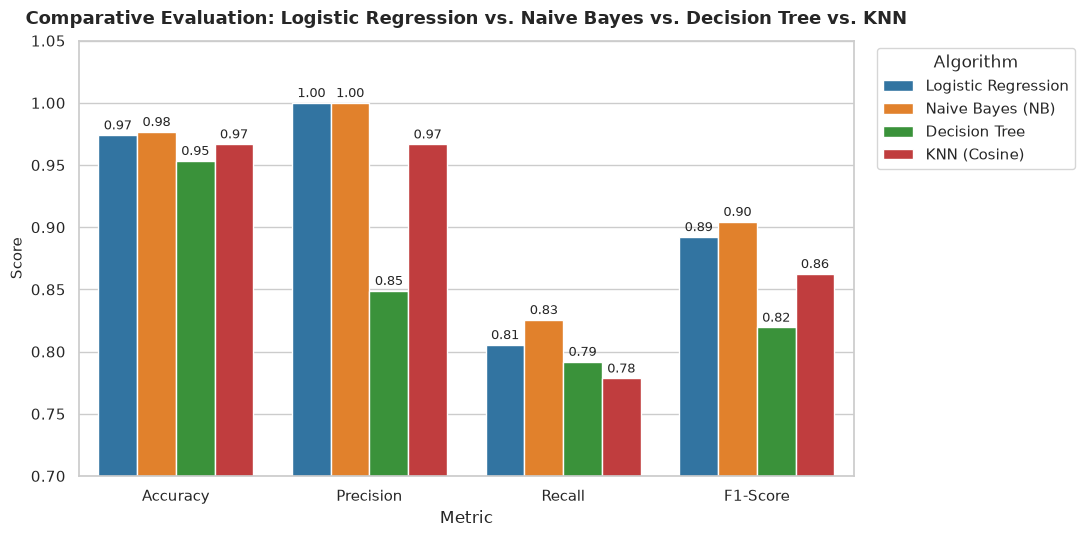
\includegraphics[width=0.88\textwidth]{figures/lr_model_comparison_bars.png}
    \caption{Comparative performance metrics (Accuracy, Precision, Recall, and F1-Score) across Logistic Regression, Naive Bayes, Decision Tree, and KNN (Cosine).}
    \label{fig:lr_bars}
\end{figure}

\begin{figure}[H]
    \centering
    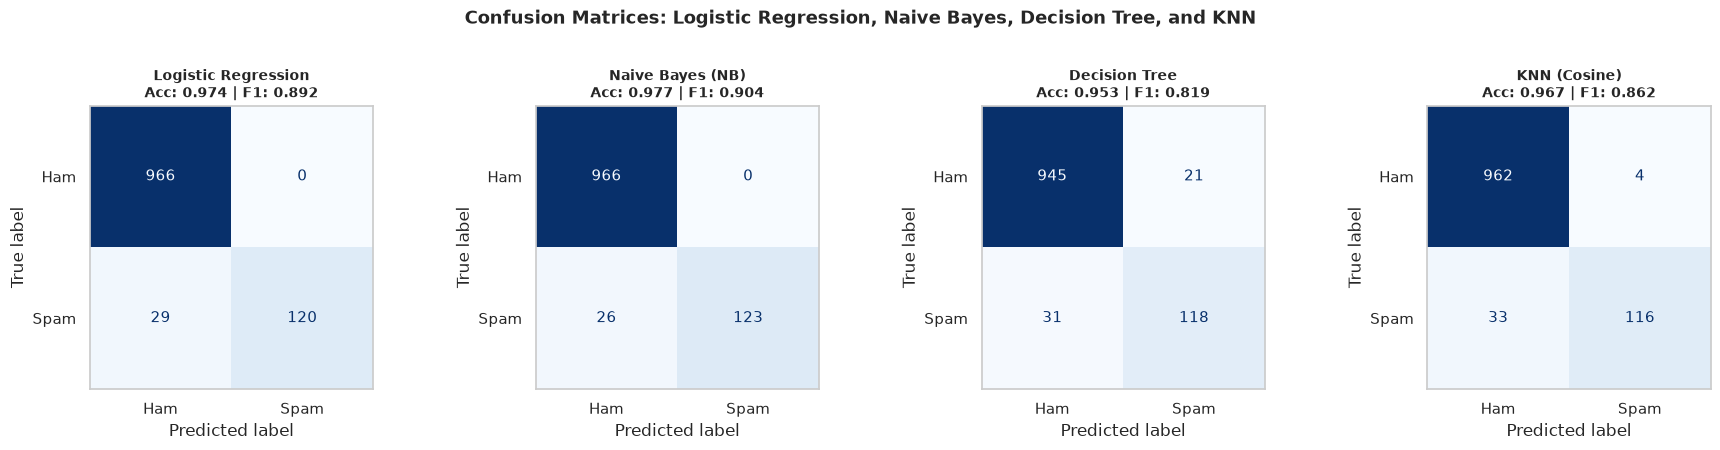
\includegraphics[width=0.98\textwidth]{figures/lr_confusion_matrices.png}
    \caption{Confusion matrix heatmaps for all four classification models on test samples ($N=1,115$).}
    \label{fig:lr_cm}
\end{figure}

\newpage
\section{In-Depth Theoretical Discussion: Generative vs. Discriminative Paradigms}

\subsection{The Precision Imperative: Zero False Positives}
In real-world SMS spam filtering, **Precision is paramount**: misclassifying a legitimate personal or transactional message as spam (a False Positive) can cause severe real-world disruption (e.g., missed OTPs or critical banking alerts). 

A key empirical finding in Table~\ref{tab:comparison_summary} and Figure~\ref{fig:lr_cm} is that:
\begin{itemize}
    \item \textbf{Logistic Regression}: Achieved a **perfect $1.0000$ Precision** ($0$ False Positives out of $966$ ham messages; $120$ True Positives, $29$ False Negatives).
    \item \textbf{Naive Bayes}: Also achieved **perfect $1.0000$ Precision** ($0$ False Positives; $123$ True Positives, $26$ False Negatives).
    \item \textbf{Decision Tree}: Incurred $21$ False Positives, dropping Precision to $0.8489$.
    \item \textbf{KNN (Cosine)}: Incurred $4$ False Positives, achieving $0.9667$ Precision.
\end{itemize}

\subsection{Generative (Naive Bayes) vs. Discriminative (Logistic Regression)}
The pairing of Naive Bayes and Logistic Regression represents a classic **Generative-Discriminative Model Pair** (Ng and Jordan, 2002):
\begin{itemize}
    \item \textbf{Generative Modeling (Naive Bayes)}: Assumes a joint probability model $P(X, Y) = P(Y) \prod_j P(X_j \mid Y)$. Naive Bayes converges to its asymptotic error rate with fewer training instances ($\mathcal{O}(\ln D)$ samples), explaining why it achieved slightly higher recall ($82.55\%$ vs. $80.54\%$) on this dataset.
    \item \textbf{Discriminative Modeling (Logistic Regression)}: Directly optimizes the conditional probability $P(Y \mid X)$ without modeling feature co-occurrences. As sample size grows ($N \to \infty$), discriminative models asymptotically surpass generative counterparts by avoiding bias introduced by violated independence assumptions.
\end{itemize}

\subsection{Why Decision Trees and KNN Underperform in Sparse Text}
\begin{enumerate}
    \item \textbf{Decision Tree Splitting Bottleneck}: Trees make axis-aligned splits on single features ($x_j \le \theta$). In text spaces with $D = 2,500$ sparse features, a single word rarely splits classes cleanly, forcing trees to construct overly deep, brittle branches that overfit noise (evidenced by $21$ False Positives).
    \item \textbf{KNN Distance Dilution}: Even when normalized on the unit sphere via Cosine distance, sparse high-dimensional exemplars suffer from hubness and equidistant distances, lowering recall to $77.85\%$.
\end{enumerate}

\section{Conclusion}
In this laboratory assignment, Logistic Regression was formulated, implemented, and benchmarked for text classification on the SMS Spam Collection corpus:
\begin{itemize}
    \item \textbf{Discriminative Precision}: Logistic Regression delivered flawless $1.0000$ precision ($0$ false alarms) and an F1-Score of $0.8922$, converging in only $19$ iterations.
    \item \textbf{Transparent Interpretability}: Feature weight coefficients provide clear linguistic explanations for classification decisions, identifying tokens like \texttt{txt}, \texttt{uk}, and \texttt{claim} as dominant spam drivers.
    \item \textbf{Linear Probabilistic Dominance}: Both linear probabilistic architectures (Logistic Regression and Naive Bayes) decisively outperformed non-linear decision trees ($95.34\%$) and metric-based KNN ($96.68\%$) in text classification.
\end{itemize}

\end{document}

